\documentclass[12pt,titlepage]{article}
\usepackage[utf8]{inputenc}
%\usepackage[czech]{babel}
\usepackage{a4wide}
\usepackage{graphicx}
\usepackage{amsmath}

\def\mathbi#1{\textbf{\em #1}}

\begin{document}

\section*{Removal of Geometric Distortion}

\begin{figure}[h]
  \centering
  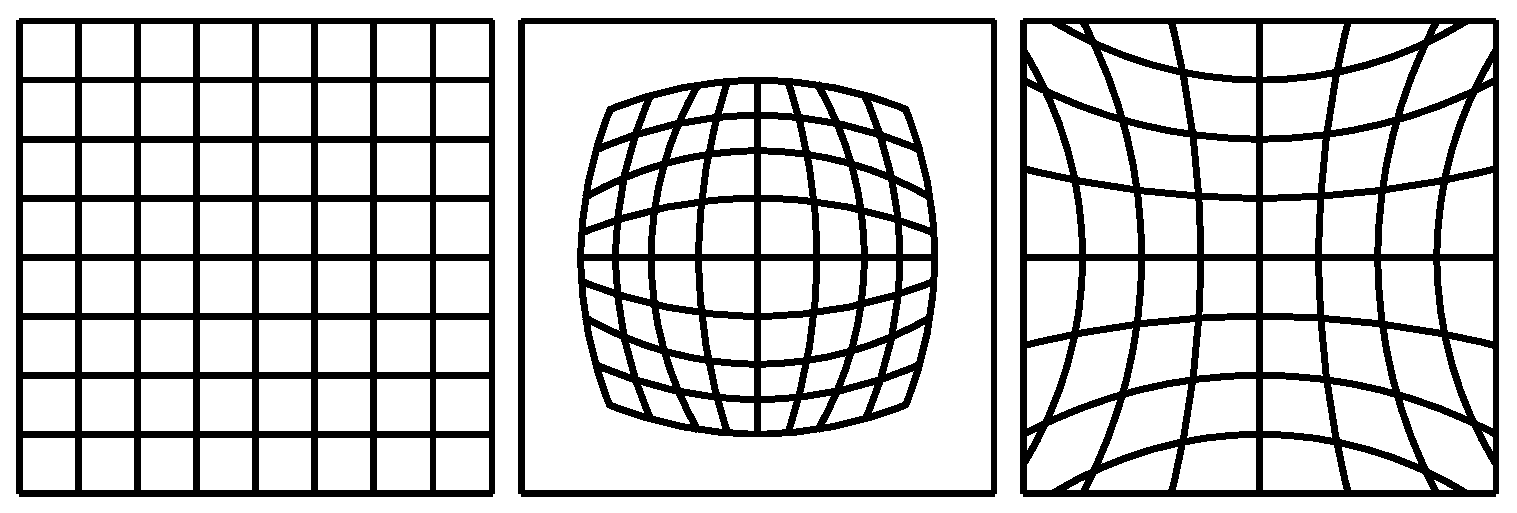
\includegraphics[width=150mm]{distortion_types.eps}
  \caption{Undistorted image, barrel distortion, and pincushion}
  \label{obr:druhy_zkresleni}
\end{figure}

%\subsection{Description of a Method}
%\label{sec:odstraneni_zkresleni}

Barrel or pincushion distortions are so called {\itshape radial} distortions. The easiest way to model such distortions is using translation of image coordinates.  Let $\bar{q} = ( x_n, y_n )^T$ represents undistorted coordinates, while $q = ( x_d, y_d )^T$ represents observed coordinates, i.e. coordinates in deformed image. Every radially symmetric distortion may be approximated using Taylor series in the following form

\begin{equation}
    \phi( r^2 ) = 1 + K_1 r^2 + K_2 r^4 + \dots,
\end{equation}
where $r^2 = \bar{x}^2 + \bar{y}^2$ a $K_1$, $K_2$, \dots are coefficients of radial distortion.

To have these coordinates independent of image dimensions, the coordinates $\bar{x}$, $\bar{y}$ are dimensionless. Moreover, to preserve radial symmetry, we must move the origin of the coordinate system to the center of image. Coordinates of required properties can be obtained using the following formula

\begin{equation}
    \label{bla1}
    \begin{array}{cc}
        \bar{x} = \frac{x_n - c_u}{R} \\
        \bar{y} = \frac{y_n - c_v}{R},
    \end{array}
\end{equation}
where $R = \sqrt{c_u^2 + c_v^2}$ and coordinates of the center of image $c_u = w / 2 $, $c_v = h / 2$ ($w$ is width and $h$ height of image).

Resulting transformation from coordinates $x_n$, $y_n$ of reconstructed image to the coordinates $x_d$, $y_d$ of original deformed image can be written using the following formula

\begin{equation}
	\label{rld:trans}
    \left( \begin{array}{c}
    x_d \\
    y_d \end{array} \right)
    =
    \left( \begin{array}{c}
    x_n - c_u \\
    y_n - c_v \end{array}\right)
    \phi^{-1}(r^2)
    +
    \left( \begin{array}{c}
    c_u \\
    c_v \end{array}\right).
\end{equation}


We go pixel by pixel of the output image $(x_n, y_n)^T$ and compute corresponding pixel coordinates in input image $(x_d, y_d)^T$. These coordinated are in general real numbers, so we have use a valid interpolation method, e.g. nearest neighbour. To achieve better result, use bilinear interpolation.


Result obtained using described method is shown in Figure \ref{rld:odstaneni_zkresleni}.

\begin{figure}
	\begin{center}
		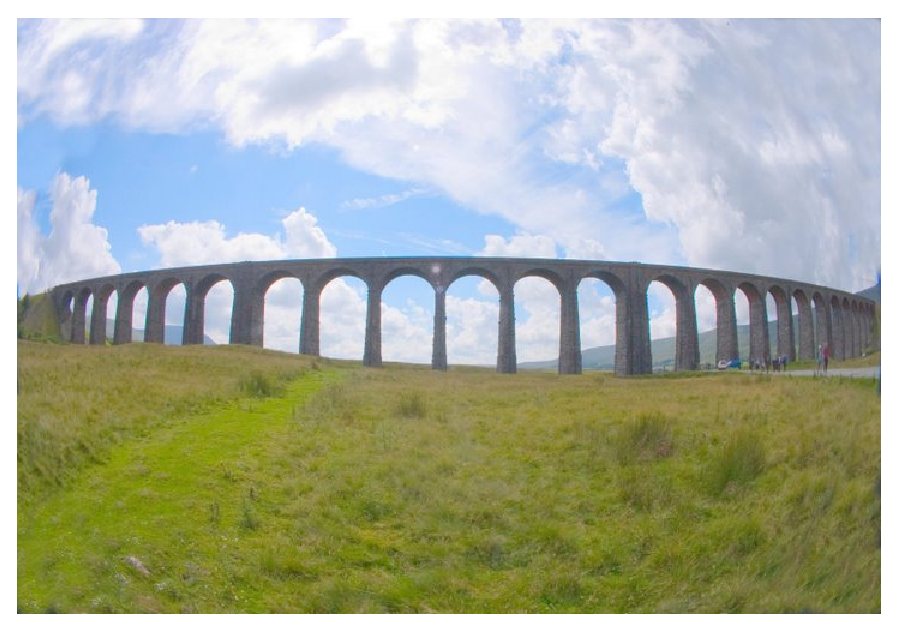
\includegraphics[scale=0.53]{distorted_image.eps}
		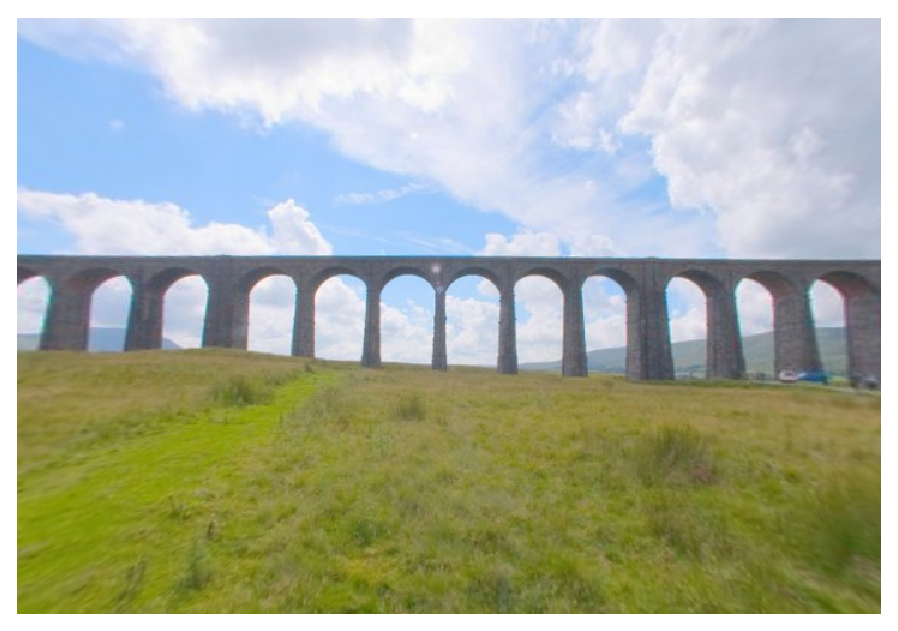
\includegraphics[scale=0.53]{human_adjusted_image.eps}
		\caption{Original distorted image (left); image after removal of radial distortion (right)}
		\label{rld:odstaneni_zkresleni}
	\end{center}
\end{figure}


\end{document}

